\section{Perturbazioni al moto Kepleriano}\linkdest{nkperturb}

\subsection{Perturbazioni del moto dei pianeti maggiori del sistema solare}

\begin{frame}{Equazione del moto e condizioni iniziali. Sistema solare.}
\begin{columns}[T]
\begin{column}{0.5\textwidth}
\begin{equation*}
\ddvec{x}_i=\sum_{\mathclap{\substack{j=0\\j\neq i}}}\frac{Gm_j}{|\vec{x}_j-\vec{x}_i|^3}(\vec{x}_i-\vec{x}_j)+\vec{a}_i
\end{equation*}
\end{column}
\begin{column}{0.5\textwidth}
\begin{block}{Source other than 9 planets newtonian interaction ($\vec{a}_i$)}
Satellites: $(m_s/m_p)(r_s/r_p)^2$.
\end{block}
\end{column}
\end{columns}
\begin{itemize}
\item General relativity. $\frac{G\msun{}}{c^2r}=\num{e-9}(\SI{1}{\astronomicalunit}/r)$.
\item Asteroids: $\num{e-9}\msun{}$. Noise.
\item Galaxy. Galaxy's tidal acceleration (ratio to Sun): $\num{e-11}(r/\SI{40}{\astronomicalunit})^3$ (negligible).
\item Passing star: tidal acceleration $\num{e-4}(r/\SI{40}{\astronomicalunit})^3$. a of most planets are adiabatic-invariants.
\item Solar mass loss. $\TDy{t}{\msun{}}=\num{e-13}\msun{}\si{\per\year}$. Slow orbital expansion (preserve relative frequencies)
\end{itemize}
\end{frame}

\begin{wordonframe}{Solar system perturbation beside 9 planet attraction}
\begin{itemize}
\item Satellites: Satellites mass is lumped in parent planet neglecting solar attraction on quadrupole moment of planet-satellite system. Fractional error (relative to solar attraction) for Moon-Earth system \num{e-7}.
\item Galaxy's Tidal acceleration: $-4\pi G\rho z\hat{z}$, $\rho\approx0.15\msun{}\si{\cubic\parsec}$ local galactic density.
\item Passing star: nearest approach at \SI{e3}{\astronomicalunit}, lasts \SI{100}{\year}.
\end{itemize}
\end{wordonframe}

\subsection{Equazioni di Gauss}

\begin{frame}{Perturbazione elementi osculanti}
\begin{block}{Forza perturbante per unit\'a di massa: $(R,W,T)$.}\end{block}
\begin{columns}[T]
\begin{column}{0.2\textwidth}
\input{osculperturb}
\end{column}
\begin{column}{0.8\textwidth}
\begin{block}{Variazione semi-assi, eccentricit\'a e inclinazione pianeti.}
\begin{align*}
&\TDy{t}{a}=\frac{2a^2}{GM}\TDy{t}{E}=\frac{2}{n\sqrt{1-e^2}}[Re\sin{f}+T(1+e\cos{f})]\\
&\xrightarrow{e\to0}\frac{2T}{n}
\end{align*}
\end{block}
\end{column}\end{columns}
\begin{align*}
&\TDy{t}{e}=\frac{1-e^2}{2ea}\TDy{t}{a}-\frac{hTa(1-e^2)}{GMea(1+e\cos{f})}\xrightarrow{e\to0}\frac{R\sin{f}2T\cos{f}}{na}\\
&\TDy{t}{i}=W\frac{\sqrt{1-e^2}\cos{(f+\omega)}}{na(1+e\cos{f})}\xrightarrow{e\to0}W\frac{\cos{(f+\omega)}}{na}
\end{align*}
\begin{columns}  \begin{column}{0.55\textwidth}
\begin{block}{Relazioni inverse}
$\Delta v_{\theta}=\frac{n\Delta a}{2}$, $\Delta v_r=na\frac{(\Delta e-\Delta a/a\cos{f})}{\sin{f}}$
\end{block}
\end{column} \begin{column}{0.45\textwidth}
\begin{block}{Drag force}
$T<0$, a diminuisce, per legge di keplero energia cinetica aumenta.
\end{block}
\end{column}\end{columns}
\end{frame}

\begin{frame}{Equazioni di Gauss: perturbazioni elementi orbitali}
\begin{block}{Variazione a e modulo di h}
\begin{align*}
&\TDy{t}{E}=Rv_r+Tv_t=[R(e\sin{f})+T(1+e\cos{f}))]\frac{Gm}{h}\\
&\TDy{t}{a}=\frac{2a^2}{Gm}\TDy{t}{E}=\frac{2}{n\eta}[T+e(T\cos{f}+R\sin{f})]\\
&\TDy{t}{h}=\PDy{a}{h}\TDy{t}{a}+\PDy{e}{h}\TDy{t}{e}=\frac{GM}{2h}[(1-e^2)\TDy{t}{a}-2ea\TDy{t}{e}]\\
\end{align*}
\end{block}
\begin{block}{Orientation of osculating plane determined by $\hat{h}$ or $(i,\Omega)$.}
$h\TDy{t}{\hat{h}}=W(\vec{r}\wedge\hat{h})$: $\hat{h}$ ruota con velocit\'a angolare $W/h\vec{r}$. Split torque into component along line of node and perpendicular to it on orbit plane: $\TDy{t}{\Omega}=\frac{rW\sin{\omega+f}}{h\sin{i}}$,
$\TDy{t}{i}=\frac{rW\cos{\omega+f}}{h}$.
\end{block}
\end{frame}

\begin{wordonframe}{Ripasso per equazioni di Gauss}
\begin{align*}
&E=-\gamma\frac{1}{2a}=-Gm_1m_2\frac{1}{2a}=-(\frac{Gm_2}{h})^2\frac{m_1}{2}(1-e^2)=-\frac{Gm_2m_1}{2a},\ \eta=\sqrt{1-e^2}\\
&h=\sqrt{GMa(1-e^2)},f:\text{ J per unit\'a di massa e anomalia vera}
\end{align*}
\end{wordonframe}

\subsection{Lagrange perturbation equations}

\begin{frame}{Lagrange perturbed equations}

\begin{block}{Lagrange's parenthesys of constant of motion is constant.}
\begin{align*}
&[F,G]=-[G,F]=\PDy{F}{q^i}\PDy{G}{p_i}-\PDy{G}{q^i}\PDy{F}{p^i}\\
&\{c_a,c_b\}[c_b,c_d]=-\delta_{ad}
\end{align*}
\end{block}
\begin{block}{Perturbing function}
Perturbing force conservative: $\vec{F}=-\nabla \phi_p$: $\TDy{t}{c_a}=\{c_a,\phi_p\}=\{c_a,c_b\}\PDy{c_b}{\phi_p}$. $H=H_0+\phi_p=\frac{1}{2}p^2-\frac{Gm}{r}+\phi_p$.
\end{block}
\end{frame}

\begin{wordonframe}{Lagrange perturbation equation}
\begin{equation*}
\phi_p(a,e,i,\Omega,\bar{\omega}=\omega+\Omega,\epsilon=\bar{\omega}+\epsilon';t), \epsilon'=nt-nt_0-\chi(t)\ \chi=\int ndt'
\end{equation*}
\begin{block}{orbital element (memo)}
\begin{columns}  \begin{column}{0.5\textwidth}
\begin{figure}[!ht]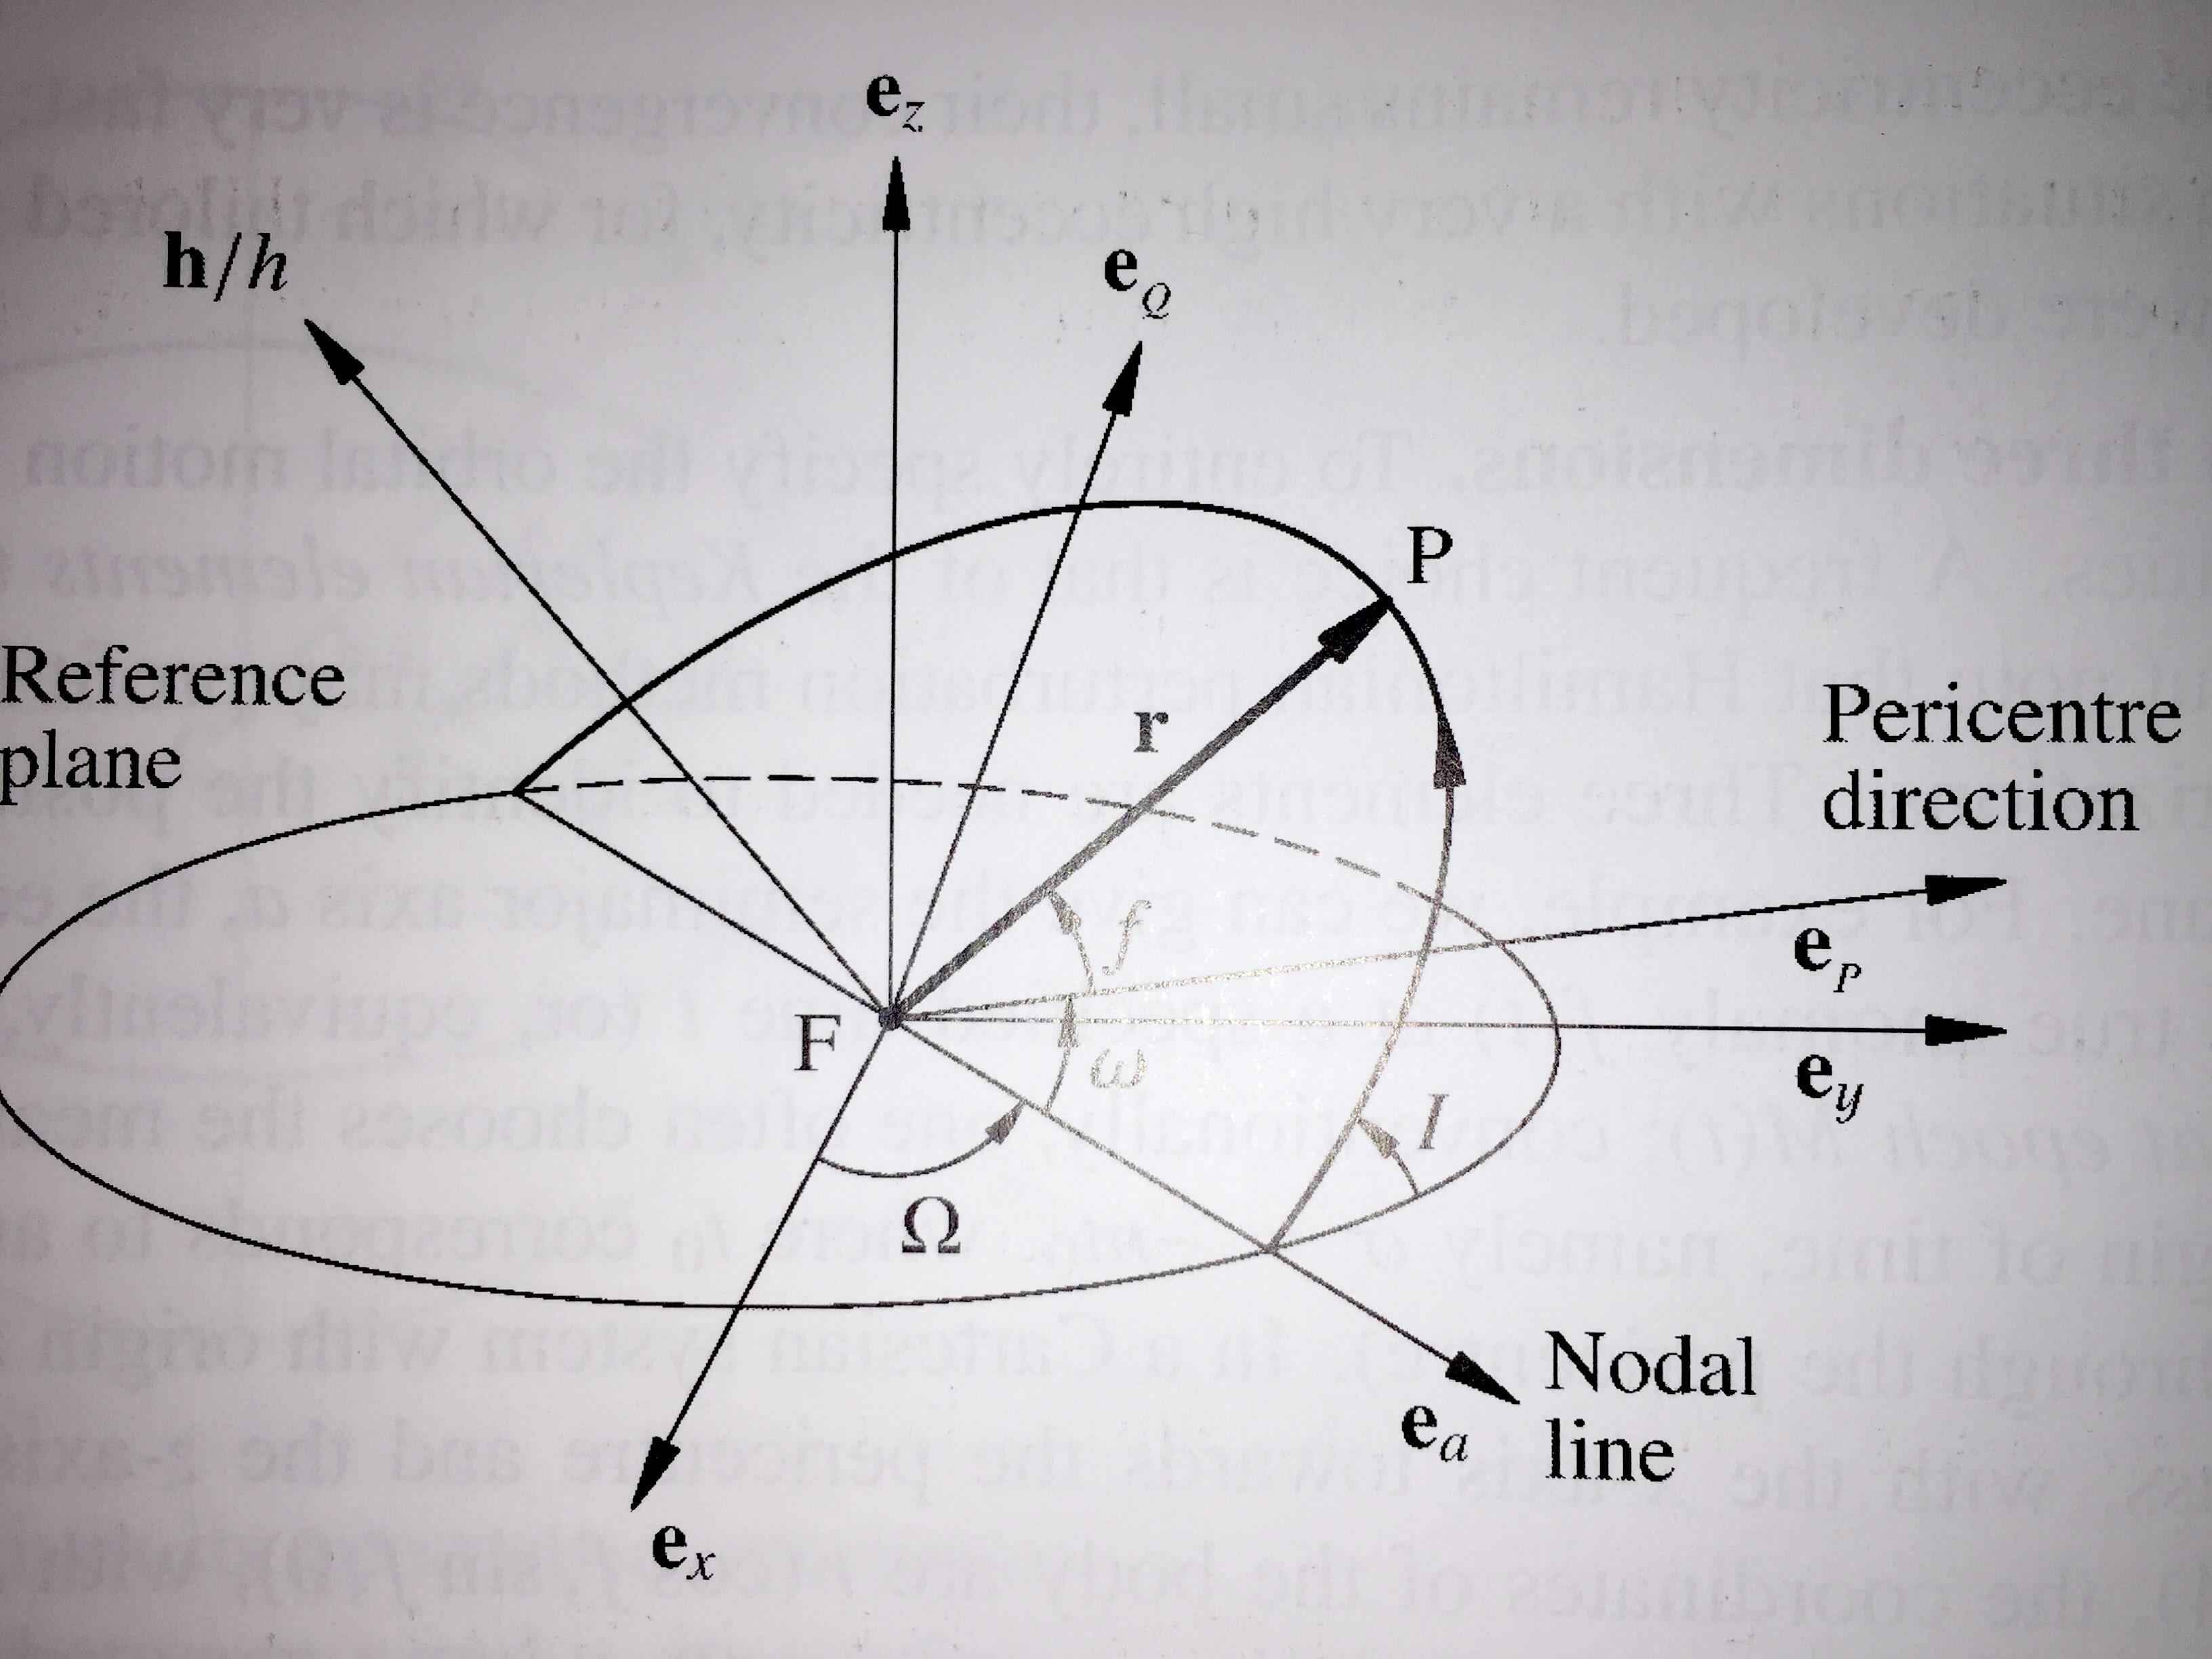
\includegraphics[width=0.95\textwidth]{orbitalbook}\end{figure}
\end{column} \begin{column}{0.5\textwidth}
\begin{align*}
&\hat{e}_P=\begin{pmatrix}\cos{\Omega}\cos{\omega}-\cos{I}\sin{\Omega}\sin{\omega}\\\sin{\omega}\cos{\Omega}+\cos{i}\cos{\Omega}\sin{\omega}\\\sin{i}\sin{\omega}\end{pmatrix}\\
&\hat{e}_Q=\hat{h}\wedge\hat{e}_P\\
&=\begin{pmatrix}-\cos{\Omega}\cos{\omega}-\cos{I}\sin{\Omega}\cos{\omega}\\-\sin{\omega}\sin{\Omega}+\cos{i}\cos{\Omega}\cos{\omega}\\\sin{i}\cos{\omega}\end{pmatrix}
\end{align*}
\end{column}  \end{columns}
\end{block}
\begin{columns}[T]\begin{column}{0.5\textwidth}
\begin{block}{Costanti del moto}
2N costanti del moto $c_a (N=3)$
\begin{align*}
\{H_0,c_a\}=0
\end{align*}
\end{block}
\end{column}\begin{column}{0.5\textwidth}
\begin{block}{Calcolo LP al pericentro)}
\begin{align*}
&\vec{r}=r[\cos{f}\hat{e}_P+\sin{f}\hat{e}_Q]\\
&\vec{v}=\frac{na}{\eta}[-\sin{f}\hat{e}_P+(e+\cos{f})\hat{e}_Q]
\end{align*}
\end{block}
\end{column}\end{columns}
\end{wordonframe}

\begin{frame}{Lagrange equation for perturbing function $\phi_p$}
\begin{align*}
&\frac{1}{a}\TDy{t}{a}=-\frac{2}{na^2}\PDy{\epsilon}{\phi_p}\\
&\TDy{t}{e}=\frac{\eta}{na^2e}[\PDy{\bar{\omega}}{\phi_p}+(1-\eta)\PDy{\epsilon}{\phi_p}]\\
&\TDy{t}{I}=\frac{1}{na^2\eta\sin{i}}[\PDy{\Omega}{\phi_p}+2\sin{i/2}(\PDy{\bar{\omega}}{\phi_p}+\PDy{\epsilon}{\phi_p})]\\
&\TDy{t}{\Omega}=-\frac{1}{na^2\eta\sin{i}}\PDy{i}{\phi_p}\\
&\TDy{t}{\bar{\omega}}=-\frac{\eta}{na^2e}\PDy{e}{\phi_p}-\frac{\tan{i/2}}{na^2\eta}\PDy{i}{\phi_p}\\
&\TDy{t}{\epsilon}=\frac{2}{na}\Dcvar{\PDy{a}{\phi_p}}{n}-\frac{\eta(1-\eta)}{na^2e}\PDy{e}        {\phi_p}-\frac{\tan{i/2}}{na^2\eta}\PDy{i}{\phi_p})
\end{align*}
%\begin{figure}[!ht]\includegraphics[height=0.45\textheight]{Lpertelem}\end{figure}
\end{frame}

\begin{frame}{Perturbazioni secolari}
\begin{columns}\begin{column}{0.5\textwidth}
\begin{block}{Perturbing function for 1 by 2}
\end{block}
\end{column}
\begin{column}{0.5\textwidth}
\begin{block}{periodic in angular variables $(\Omega_1,\bar{\omega}_1, \lambda_1; \Omega_2,\bar{\omega}_2, \lambda_2)$}\end{block}
\end{column}  \end{columns}
\begin{align*}
\phi_p=-Gm_2(\frac{1}{r_{12}}-\frac{\vec{r}_1\cdot\vec{r}_2}{r_2^3})\qquad\to\qquad \sum C_{ijk}\cos{\Phi_{ijk}}
\end{align*}
\begin{block}{Rate of change of elements of j-planets due to i}
\begin{align*}
&\mu=\frac{\phi_p}{Gm/a}=\frac{\phi_p}{n^2a^2}>=\frac{a_p}{n^2a}\\
&\TtwoDy{t}{\chi}\approx O(\mu n^2),\ \TDy{t}{c_i}(\frac{\dot{a}}{a}\approx O(\mu n)
\end{align*}
$a$ are stable to $\mu^2$ (Lagrange/Tisserand):no secular term over $\frac{1}{\mu^2}$ orbital period.
\end{block}
\begin{block}{mean orbital elements}
\begin{align*}
&(\TDy{t}{\vec{c}'_j})_i=\mu\exv{F_{ji}}=\frac{\mu}{(2\pi)^2}\iint^{2\pi}\,d\lambda_i\,d\lambda_j\mu F_{ji}(\vec{c}'_j,\lambda_j,\vec{c}'_i,\lambda_i)
\end{align*}
\end{block}
\end{frame}

\begin{wordonframe}{Perturbazioni elementi orbitali}
$\Dcvar{\TDy{t}{\vec{c}_a}}{i}=f_a(c_b(t),t)$, orbital phase $\TtwoDy{t}{\chi}$
\begin{align*}
&\vec{c}_i=(a_i,e_i,i_i,\bar{\omega}_i,\Omega_i,\epsilon_i)\\
&\lambda_i\text{: mean longitude}\leftrightarrow \chi=\int\,dt’\chi
\end{align*}
Perturbation function for planet 1
\begin{align*}
&\TtwoDy{t}{\vec{r}}=-G(\msun{}+m_1)\frac{\vec{r}_1}{r_1^3}+Gm_2(\frac{\vec{r}_2-vec{r}_1}{r_{12}^3}-\frac{\vec{r}_2}{r_2^3})\\
&=-\PDof{\vec{r}_1}[-\frac{G(\msun{}+m_1)}{r_1}+\phi_p]\\
&\phi_p=\sum C_{ijk}\cos{(i_1\lambda_1+i_2\lambda_2+j_1\bar{\omega}_1+j_2\bar{\omega}_2+k_1\Omega_1+k_2\Omega_2)}
\end{align*}
\end{wordonframe}

\section{Secular theory.}\linkdest{secular}

\begin{frame}{Secular planetary theory ($\phi_p$ linearized in e,i)}
\begin{columns}[T]\begin{column}{0.5\textwidth}
\begin{block}{Non-singular elements}
\begin{align*}
&h=e\sin{\bar{\omega}},\ k=e\cos{\bar{\omega}}\\
&P=\sin{i}\sin{\Omega},\ Q=\sin{i}\cos{\Omega}
\end{align*}
\end{block}
\end{column}\begin{column}{0.5\textwidth}
\begin{block}{L perturbation equation linear in e,i (Long-term evolution)}
\begin{align*}
&\TDy{t}{h}=-\frac{1}{na^2}\PDy{k}{\phi_p},\ \TDy{t}{k}=\frac{1}{na^2}\PDy{h}{\phi_p}\\
&\TDy{t}{P}=-\frac{1}{na^2}\PDy{Q}{\phi_p},\ \TDy{t}{Q}=-\frac{1}{na^2}\PDy{P}{\phi_p}
\end{align*}
\end{block}
\end{column}\end{columns}
\begin{block}{Lagrange (linear) solution}
\begin{columns}[T]\begin{column}{0.5\textwidth}
\begin{align*}
&h_i=\sum_jR_{ij}\sin{(g_jt+\beta_j)},\\
&k_i=\sum_jR_{ij}\cos{(g_jt+\beta_j)}\\
&P_i=\sum_jS_{ij}\sin{(s_jt+\gamma_j)},\\
&Q_i=\sum_jS_{ij}\cos{(s_jt+\gamma_j)}
\end{align*}
\end{column}
\begin{column}{0.5\textwidth}
\begin{block}{ND harmonic oscillator}
\begin{align*}
&\TtwoDy{t}{\vec{h}'}=-B'^2\cdot\vec{h}',\ldots
\end{align*}
\end{block}
$g_j, s_j\approx O(\mu n)$ typ. period \SI{50}{\kilo\year}-few \si{\mega\year}, i,j from 1-N but labels modes not planets.
\begin{align*}
\sum_jm_jn_ja_j^2(h_j^2+k_j^2)=\sum_jm_jn_ja_j^2e_j^2=\const{}
\end{align*}
\end{column}\end{columns}
\end{block}
\end{frame}

\begin{wordonframe}{Secular planetary theory}
In solar system e,i are small $\approx \sqrt{\mu}$; $\vec{e}_i\cdot\vec{e}_j=h_ih_j+k_ik_j$.
\begin{align*}
&W_{ij}=m_j\exv{R_{ij}}=-[B_{ij}(h_ih_j+k_ik_j)+\frac{1}{2}B_{ii}(h_i^2+h_j^2+k_i^2+k_j^2)\\
&+C_{ij}(P_iP_j+Q_iQ_j)+\frac{1}{2}C_{ii}(P_i^2+P_j^2+Q_i^2+Q_j^2)]\\
&m_i,\vec{h}=h_i,\ldots\\
&h_i'=\sqrt{m_in_ia_i^2}h_i,\ k_i'=\sqrt{m_in_ia_i^2}k_i,\ B_{ij}'=B_{ij}/\sqrt{(m_jn_ja_j^2)(m_in_ia_i^2)}
\end{align*}
Lagranage equation in Hamiltonian form:
\begin{equation*}
\TDy{t}{\vec{h}'}=B'\cdot\vec{k}'\quad\TDy{t}{\vec{k}'}=-B'\cdot\vec{k}'
\end{equation*}
\begin{block}{secular resonances}
\begin{columns}[T]\begin{column}{0.6\textwidth}
located in surface in $(a,e,i)$ space: $g-g_i=0$ ($\nu_i$), $s-s_j=0$ ($\nu_{1j}$). When the forced contribution prevails values of some elements of a test body are determined by whole planetary dynamics. $g=B_{00}/(mna^2)$
\end{column}\begin{column}{0.4\textwidth}
\begin{figure}[!ht]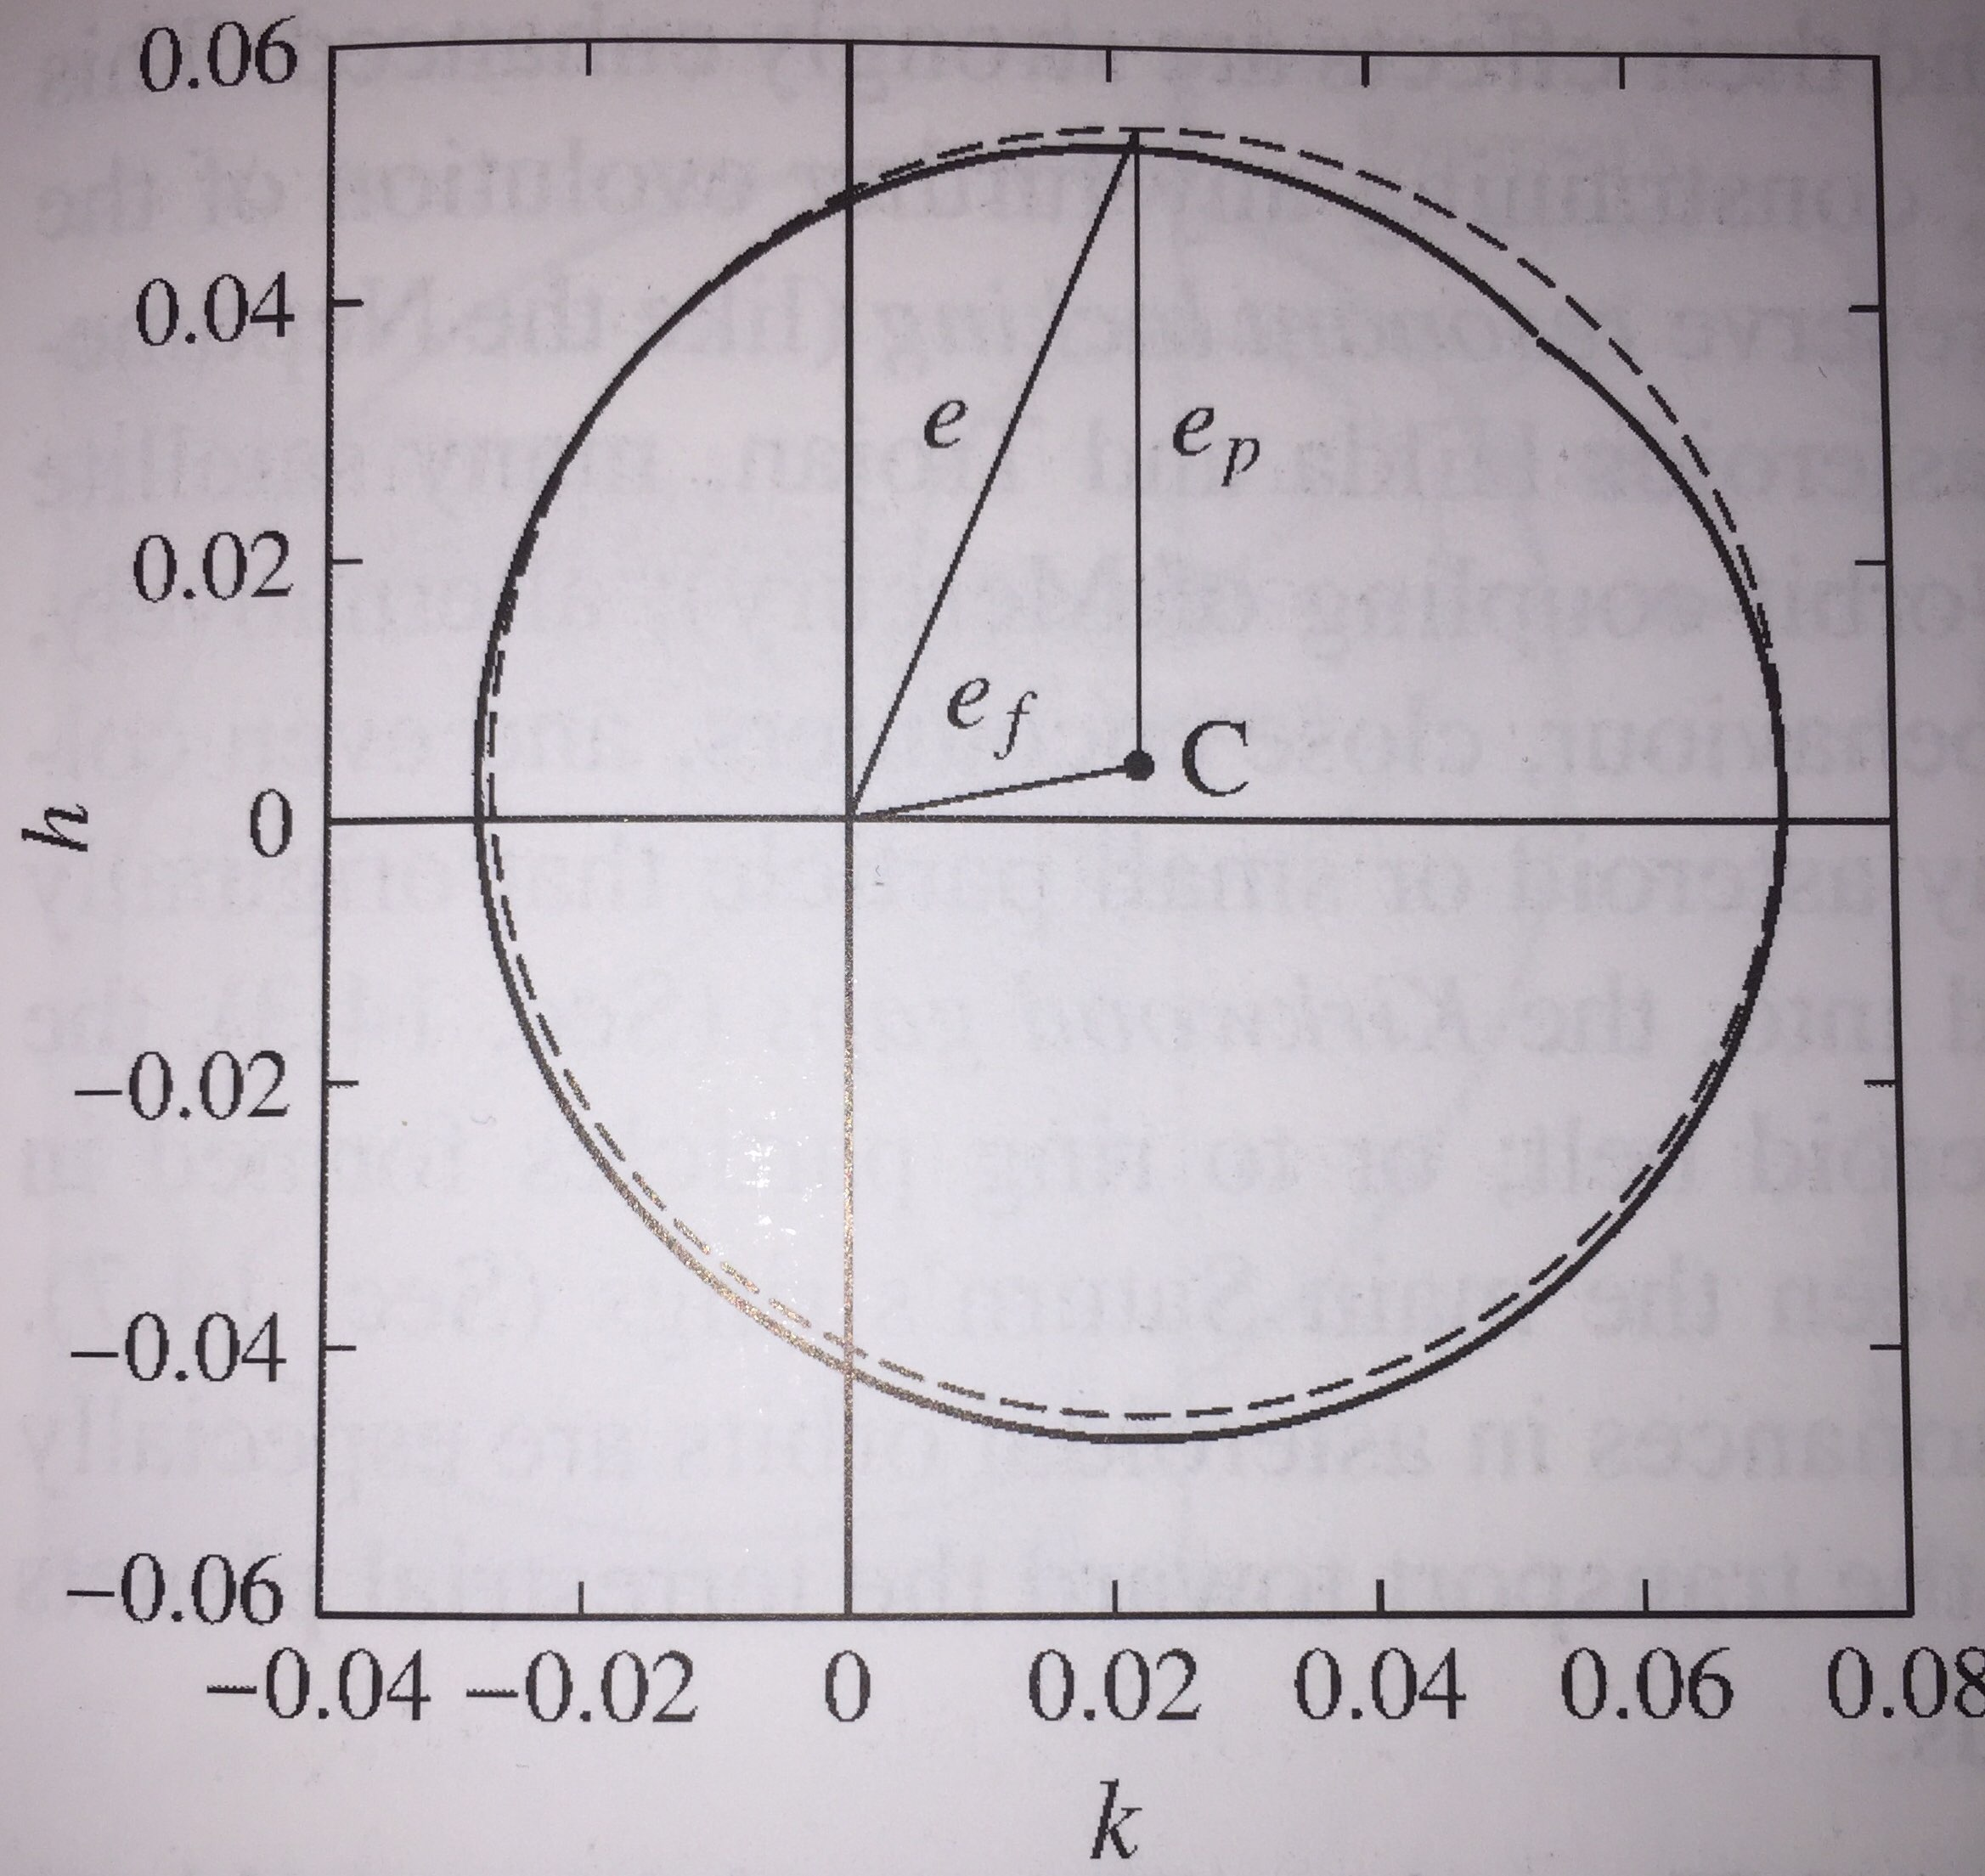
\includegraphics[keepaspectratio,width=0.7\textwidth]{forcedres}\end{figure}
\end{column}\end{columns}
\end{block}
\end{wordonframe}

\section{Resonances and chaotic evolution.}\linkdest{resonanceschaos}

\begin{frame}{Resonances and ergodic behaviour}
\begin{columns}[T]
\begin{column}{0.45\textwidth}
\begin{figure}[!t]
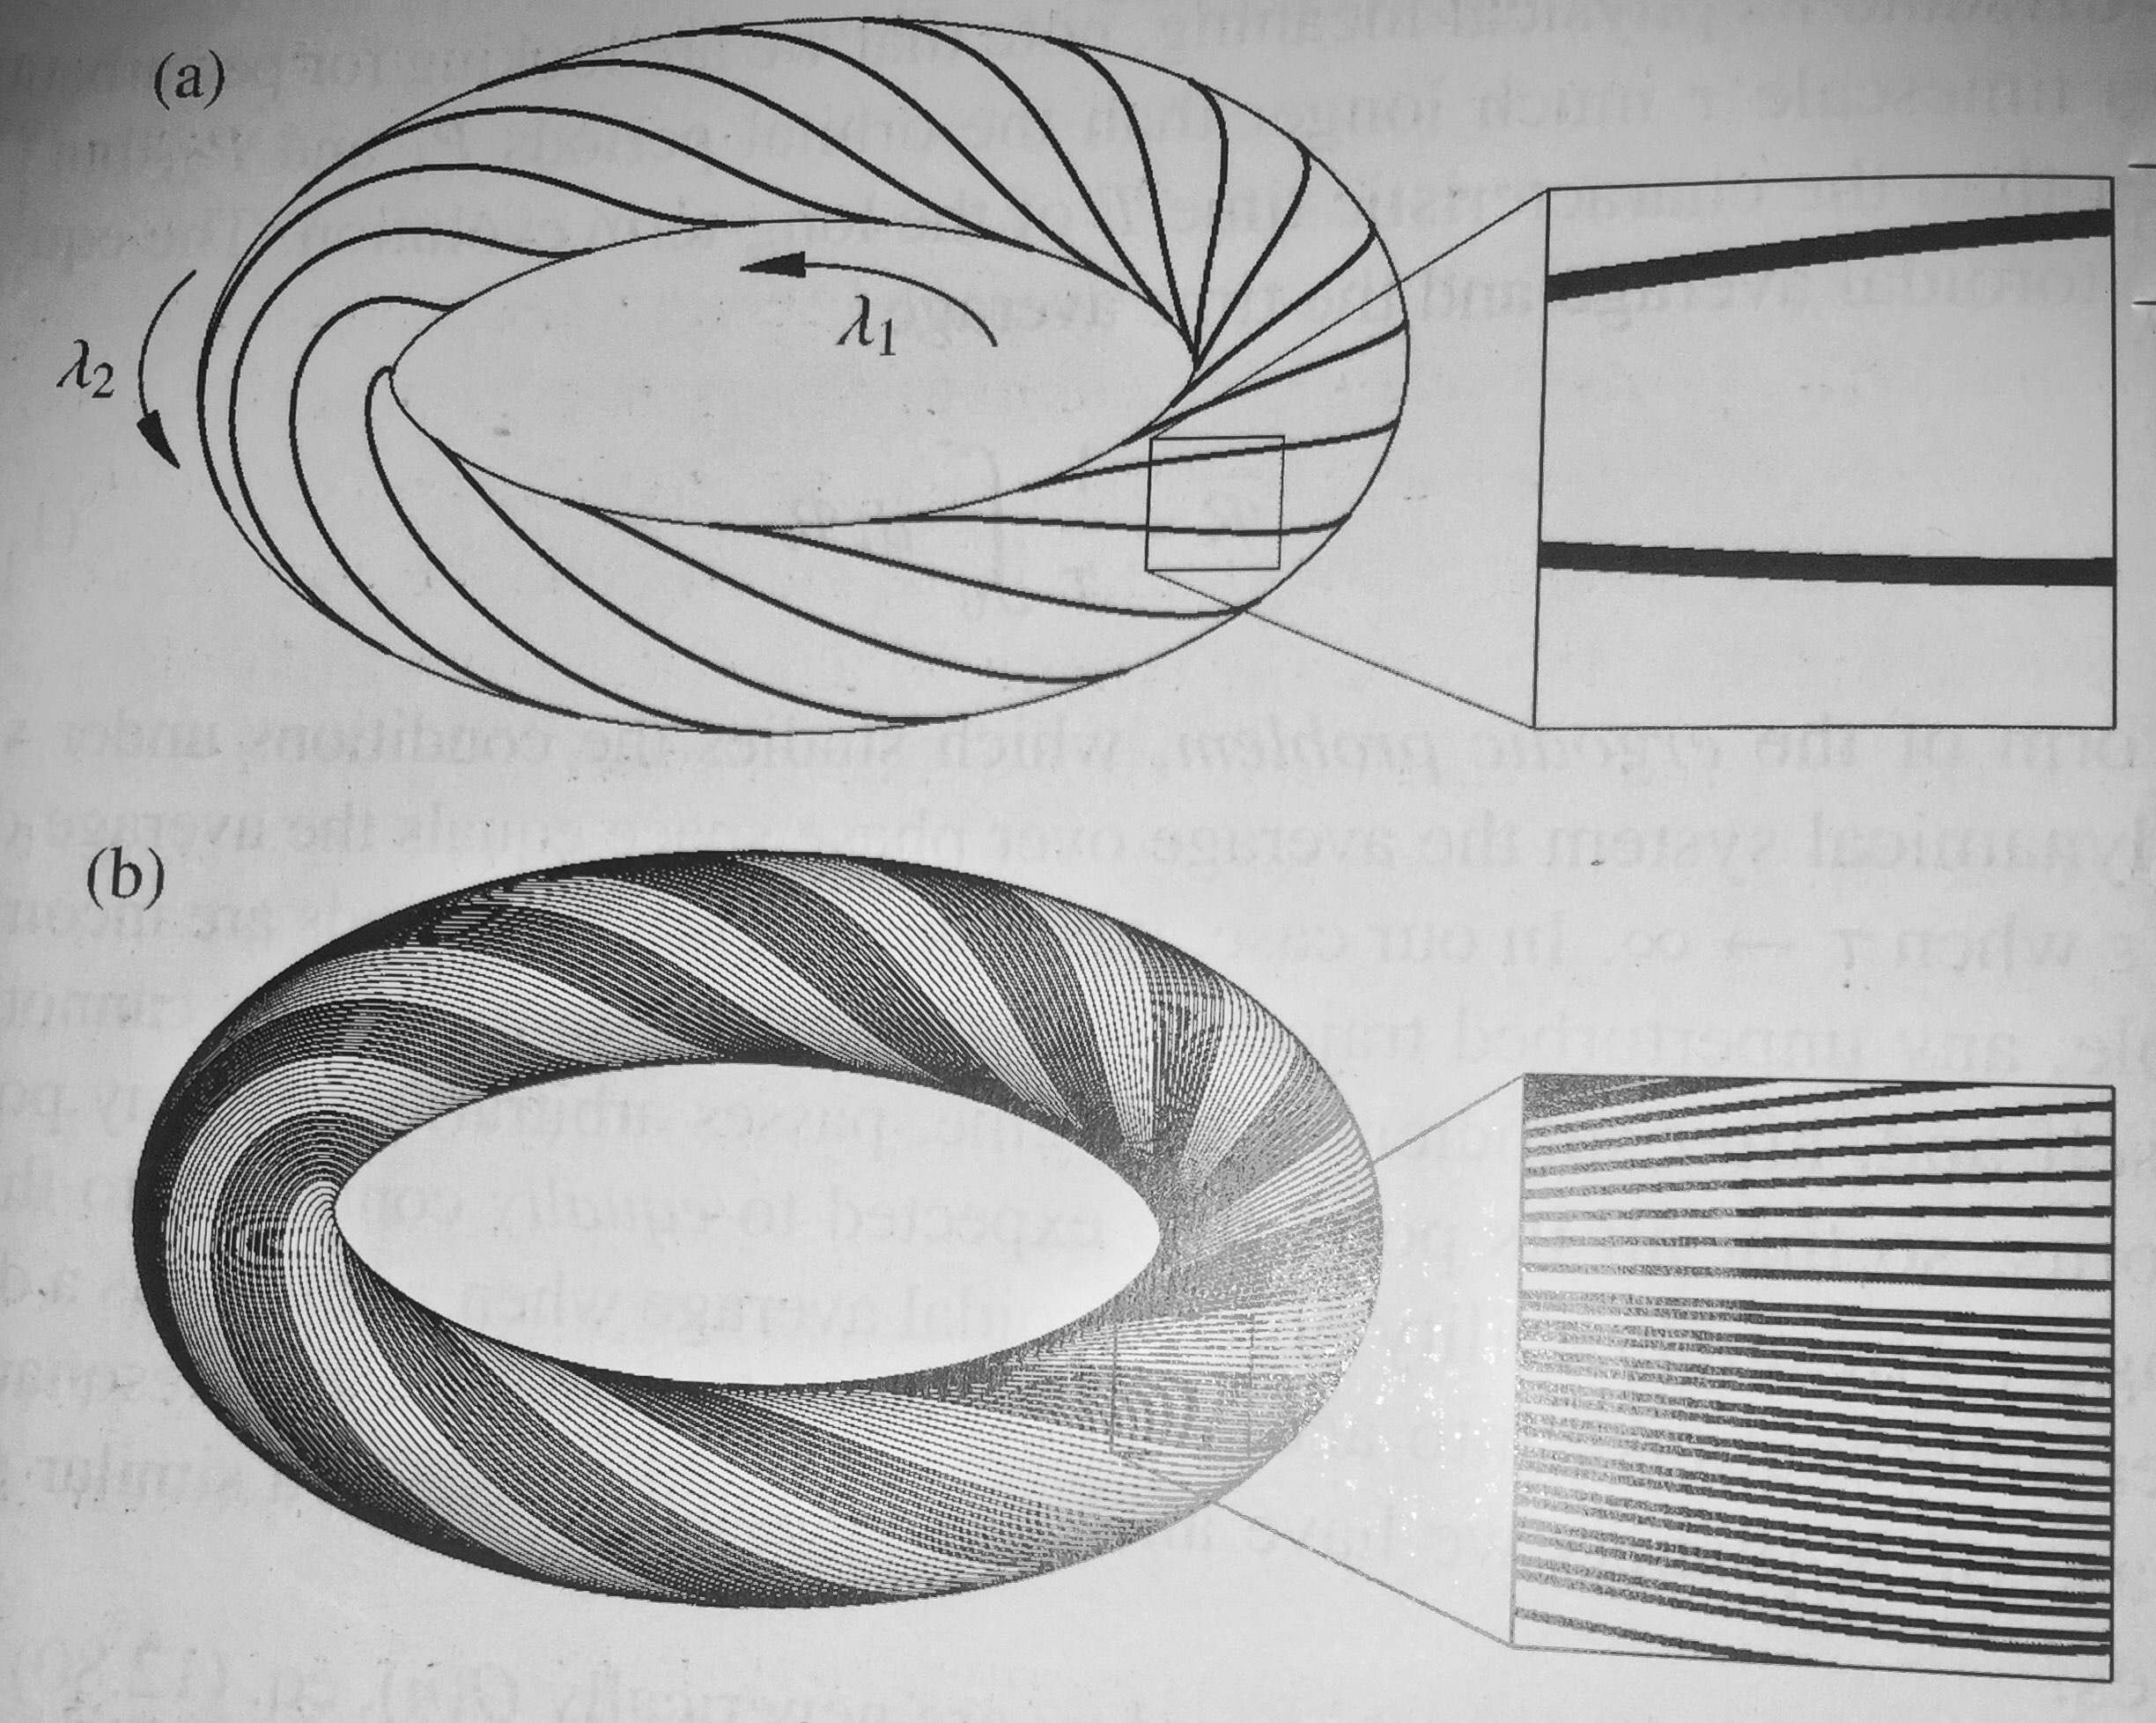
\includegraphics[width=0.9\textwidth]{resergo}
\end{figure}
Resonance condition (risonanze di moto medio): $i_1n_1+i_2n_2=0$.
secular effects (beyond lowest order in $\mu$):
\begin{align*}
&i_1(n_1+\dot{\epsilon}_1)+i_2(n_2+\dot{\epsilon}_2)+j_1\dot{\bar{\omega}}_1+j_2\dot{\bar{\omega}}_2\\
&+k_1\dot{\Omega}_1+k_2\dot{\Omega}_2=0
\end{align*}
\end{column}
\begin{column}{0.55\textwidth}
\begin{block}{Periodic pertutbation}
\begin{align*}
\bar{\phi_p}=\frac{1}{\tau}\int_0^{\tau}\phi_p\,d\tau
\end{align*}
elliptic orbit around oblate planet
\end{block}
\begin{block}{Non-periodic problem}
Two-planet system: average over torus $(\lambda_1,\lambda_2)$: $\exv{\phi_p}_{torus}$.
\end{block}
\end{column}
\end{columns}
\end{frame}

\begin{wordonframe}{Resonance and ergodicity}
\begin{block}{Torus in phase space: KAM theorem}
Figure: behaviour of $\phi_p$ for two body around primary (periodic) for resonant/non resonant case.
\begin{align*}
\exv{\phi_p}_{torus}=\frac{1}{(2\pi)^2}\int_0^{2\pi}d\lambda_1\,d\lambda_2\phi_p(\lambda_1,\lambda_2,\ldots)
\end{align*}
\end{block}
Ergodic problem: condition in dynamical system when average over phase space equal average over time to infinity.
A phase $\phi$ in $ C_{ijk}\cos{\Phi_{ijk}}$ is stationary: integrli del coseno crescono linearmente; non \'e valida ipotesi ergddica (equation for resonance including secular effects)
Secular resonance: $i_1=i_2=0$ ($\nu_6$ fascia asteroidale).
(Mimas and Tetis: tidal evolution have driven satellite from a multiplet line to another)
Risonanze: congelano stato dinamico o evoluzione caotica
\end{wordonframe}

\begin{frame}{Chaotic behaviour}
\begin{block}{Regime caotico}
Condizioni iniziali arbitrariamente vicine possono dar luogo a soluzioni molto diverse per grandi t.
Divisione spazio delle fasi in regione regolare e caotica.
\end{block}
\begin{block}{Esponente di Lyapunov}
The distance between two trajectories in phase space initially distant $\delta \gamma_0$ evolves $|\gamma(t)|=\delta\gamma_0\exp{\lambda t}$. $\lambda>0$ regime caotico (Lorenz 1963)

\end{block}
\end{frame}

\begin{wordonframe}{Comportamento caotico}
\begin{itemize}\item Mappa logistica: $x_{n+1}=Ax_n(1-x_n)$, per $A>3.57$ andamento caotico.
\item Ruota di Lorenz.
\begin{align*}
&\TDy{t}{m}=Q-km-\PDy{t}{m}\\
&m(\theta,t)=\sum_0^{\infty}[a_n(t)\sin{(n\theta)}+b_n(t)\cos{(n\theta)}]\\
&I\TDy{t}{\omega}=-\nu\omega+gr\int_0^{2\pi}m(\theta,t)\sin{\theta}\,d\theta=-\nu\omega+(\sum)\pi gra_n\\
&\TDy{t}{a_n}=n\omega b_n-Ka_n,\ \TDy{t}{b_n}=-n\omega a_n-Kb_n
\end{align*}
\end{itemize}
\end{wordonframe}

\begin{frame}{Tidal interaction}
\begin{block}{Darwin-Mignard tidal model (mignard81)}
\begin{align*}
&\vec{f}=-3k_2\Delta t \frac{Gm_1^2R_0^5}{r\expy{10}}[2\vec{r}\scap{r}{v}+r^2(\vecp{r}{\Omega}+\vec{v})]\\
&\ddvec{r}=-\frac{GM}{r^3}\vec{r}+\frac{\vec{f}}{m}\\
&\vec{T}=-\vecp{r}{f}=I\dvec{\Omega}=3k_2\Delta t \frac{Gm_1^2R_0^5}{r^8}[r^2\vec{\Omega}-\scap{r}{\Omega}\vec{r}+\vecp{v}{r}]
\end{align*}
\end{block}
\end{frame}

\section{Effetti dinamici della radiazione}\linkdest{radiation}

\begin{frame}{Effetti della Radiazione}
\begin{columns}[T]\begin{column}{0.5\textwidth}
\begin{block}{Radiation/Gravity ratio}
$\beta=\frac{F_{rad}}{F_g}\propto\frac{S}{m}\approx\frac{\num{5.8e-5}}{\rho R}\approx\num{3e-10}$ ($R\approx\SI{1}{\kilo\meter}$, $\rho\approx\SI{1}{\gram\per\cubic\cm}$).
$G\msun{}\to(1-\beta)G\msun{}$.
\end{block}
\begin{block}{Variazione semiasse}
Equazione di Gauss: $\TDy{t}{a}=\frac{2T(a)}{n(a)}\propto a^{-2}a\expy{-\frac{3}{2}}\propto a\expy{-\frac{1}{2}}$.
\end{block}
\end{column} \begin{column}{0.5\textwidth}
\begin{block}{Effetto Poynting-Robertson}
Radiation force
\begin{equation*}
\vec{f}=Q_{pr}\frac{FS}{c}[(1-\hat{n}\cdot\frac{\vec{v}}{c})\vec{n}-\frac{\vec{v}}{c}]
\end{equation*}
Timescale of orbital circularization and decay: $\tau_d\approx\frac{mc^2}{FS}\approx\num{7e-6}(\frac{\rho}{\si{\gram\per\cubic\cm}})(\frac{R}{\si{\cm}})(\frac{r}{\si{\astronomicalunit}})^2\si{\year}$.
\end{block}
\end{column}  \end{columns}
\begin{block}{Effetto Yarkovsky}
Radiative recoil: l'effetto Y. \'e prodotto dal riscaldamento inomogeneo causato da una sorgente esterna.
$T_s=T_{eq}+\Delta T_s$. Infinite plane with periodic heat flux (toy model): $\Delta T_s\propto\exp{2\pi\nu t+\phi_t}$, temperature lags behind  flux.
Y recoil acceleration:
\begin{equation*}
\vec{f}_Y=-\frac{2}{3}\frac{\epsilon\sigma}{mc}\int_S\,dS\vec{n}_{\bot}T_s^4\approx-\frac{8}{3}\frac{\epsilon\sigma}{mc}T_{eq}^3\int_S\,dS\vec{n}_{\bot}\Delta T_s
\end{equation*}
\end{block}
\end{frame}

\begin{wordonframe}{Evoluzione dinamica: Effetti radiazione}
\begin{block}{Effetto Poynting-Robertson}
Radiation pressure: term $\propto\frac{1}{c}$.
$Q=Q_{ab}+gQ_{sc}$: g tiene conto dell'asimmetria tra forward/backward scattering.
\end{block}
\begin{block}{Effetto Yarkovsky}
Rotazione prograda/retrograda: accelerazione/decelerazione (a aumenta/diminuisce). Introduce rumore nella distribuzione nello spazio degli elementi orbitali delle famiglie dinamiche degli asteroidi.
\begin{equation*}
\tan{\phi_t}=-\frac{\Theta}{1+\Theta},\quad \Theta=\frac{\rho c_P\sqrt{\pi\chi\nu}}{4\epsilon\sigma T_{eq}^3}
\end{equation*}
Per corpèi inferiori al metro la conduzione riduce Yarkovsky.
Important for small NEO; a meteoroid (decine di metri): $\Delta a\approx 0.1\si{\astronomicalunit}$ (mean distance to Kirkwood gap) in few tens of \si{\mega\year}; a kilometer size asteroid: $\Delta a\approx 0.01\si{\astronomicalunit}$ (width of asteroid family) in \si{\giga\year}.
Eccesso NEO retrogadi: popolati da risonanze $\nu_6$ (bordo interno) e $3:1$ (intermedia) con uguale peso: dalla prima asteroidi che diminuiscono a.
\end{block}
\end{wordonframe}

\begin{frame}{Effetto YORP. Vento solare. Interazioni EM.}
\begin{block}{effetto YORP}\end{block}
\begin{columns}[T]\begin{column}{0.5\textwidth}
Oggetto di forma irregolare ($R<\SI{10}{\kilo\meter}$): trasferimento momento angolare (radiazione riflessa).
\end{column}
\begin{column}{0.5\textwidth}
\begin{align*}
&\TDy{t}{\omega}=\frac{\tau_z}{c}\\
&\TDy{t}{\theta}=\frac{\tau_{\theta}}{c\omega}\\
&\theta<(>)\deg{55}: \omega \uparrow(\downarrow)
\end{align*}
\end{column}  \end{columns}
\begin{block}{Solar wind}
Momentum flux $\propto\frac{1}{r^2}$: \num{3e-4} times smaller than radiation pressure. Drag ($\frac{v}{c}\to\frac{v}{v_w}$): $0.3$ times the Poynting-Robertson drag.
\end{block}
\begin{block}{EM interactions}
Ionization by UV, flux of electrons/ions. 
\end{block}
\end{frame}

\begin{wordonframe}{Effetto YORP. Vento solare. Interazioni EM. (e recap)}
\begin{block}{Effetto YORP}
\begin{align*}
d\vec{\tau}=\vec{r}\wedge\vec{f\,dA},\ \vec{f}=-\frac{2F_S\cos{\theta}\hat{n}}{3c}
\end{align*}
(Rubincam 2000). Rende gli assi ortogonali al piano orbitale.
\end{block}
\begin{block}{Solar wind}
$\rho_W\approx\SI{e-23}{\gram\per\cubic\cm}$, $v_W\approx\SI{400}{\kilo\meter\per\second}$.
\end{block}
Addensamento al bordo dello spazio degli elementi orbitali.
La dimensione dell'oggetto determina la velocit\'a di migrazione: stima et\'a delle famiglie.
\begin{block}{Solar wind}
For particles smaller than \SI{0.1}{\micro\meter} orbital decay is mainly due to solar wind drag.
\end{block}
\begin{block}{EM interactions}
A body in a plasma with $n_e$ charges negative until $\phi_e\approx KT/e$ restore equilibrium (extended over distance $\lambda_D$): for body smaller than \SI{1}{\micro\meter} is relevant Lorentz acceleration $qvB/(mc)\propto\frac{1}{R^2}$.
Planetary rings: particles motion is influenced by surrounding plasma and planet magnetic field. (Lorentz resonances: magnetic field frequency commensurable to particle's epicyclic frequencies).
\end{block}
\end{wordonframe}


\subsection{Evoluzione dinamica del sistema sistema solare. Stabilit\'a.}

\begin{frame}{Simulazioni}

\end{frame}
\begin{wordonframe}{simulazioni numeriche}

\end{wordonframe}
        